\section{Model}

\begin{equation}
    \textbf{State space: }\statespace = \R^{2} \times \{0, 1, 2, 3, 4, 5\} \times \{ 18, 19, \cdots , 84, 85\}
\end{equation}

\begin{equation}
    \textbf{Action space: }\actionspace  = \{0, 15, 25, 37, 45\}
\end{equation}

\begin{equation}
    \textbf{States: }\{A, Z, K, Q\}, \qquad \textbf{Actions: } \{H\} 
\end{equation}

\begin{equation}
    \textbf{Variables: }\{L, W, Y, C, B, U\},  \qquad \textbf{Parameters: } \{\kappa, \mu_\rho, \sigma_\rho, p_\psi, \sigma_\epsilon, \zeta, a, b, c, d\}
\end{equation}

The variables are normalized such that their values correspond to a single week. I.e. the agent can choose to work between 0 and 45 hours a week. The agents consumption will be normalized to weekly levels. The state $M$ represents Cash-on-hand, the sum of assets and salary. $Z$ is the idiosyncratic wage level. $K$ is the number of kids and $Q$ is the age of the agent. In this formulation time $(t)$ and age $(Q)$ are explicitly modelled separately, such to clearly separate what is a function of age and what is a function of time. f.x. The wage level is modelled to follow a certain pattern as a function of age, not of time. Importantly for solving the model, I do not need to integrate out the age since it is perfectly deterministic. The action space contains a single discrete variable $H$ that denotes the number of working hours.

Model dynamics:

\begin{align}
    U_t (C_t, L_t, B_t) &= C_t^{1-B_t}L_t^{B_t} \label{eq:utility_v1}\\
    B_t (K_t) &= f^{B}(K_t) \label{eq:alpha_v1}\\
    Y_t ( H_t, W_t) &= H_t \cdot W_t \label{eq:salary_v1}\\
    C_t (A_t, Y_t) &= \kappa \cdot (A_t + Y_t) \label{eq:consumption_v1}\\
    L_t(H_t) &= 7 \cdot 24 - H_t \label{eq:leisure_v1}\\
    W_t(Z_t, Q_t) &= f^{W_t}(Q_t) + Z_t \label{eq:wage_v1}
\end{align}

Law of motion (transitionsligninger XXX):

\begin{align}
    A_{t+1}(A_t, Y_t, C_t) &= \rho_{t+1} \cdot (A_t + Y_t - C_t), \qquad \rho_{t+1} \sim \ndist(\mu_{\rho}, \sigma_{\rho}) \label{eq:assets_v1} \\
    K_{t+1} (K_t) &= K_t + \psi_{t+1}, \qquad \psi_{t+1} \sim Bernoulli(p_{\psi}) \label{eq:kids_v1}\\
    Z_{t+1} (Z_{t}) &=  \zeta \cdot Z_t \cdot \epsilon_{t+1} \qquad \log (\epsilon_{t+1} ) \sim \ndist(0, \sigma_{\epsilon}) \label{eq:wage_level_v1}\\
    Q_{t+1} (Q_t)&= Q_t + 1 \label{eq:age_v1}
\end{align}

\begin{figure}
    \centering
    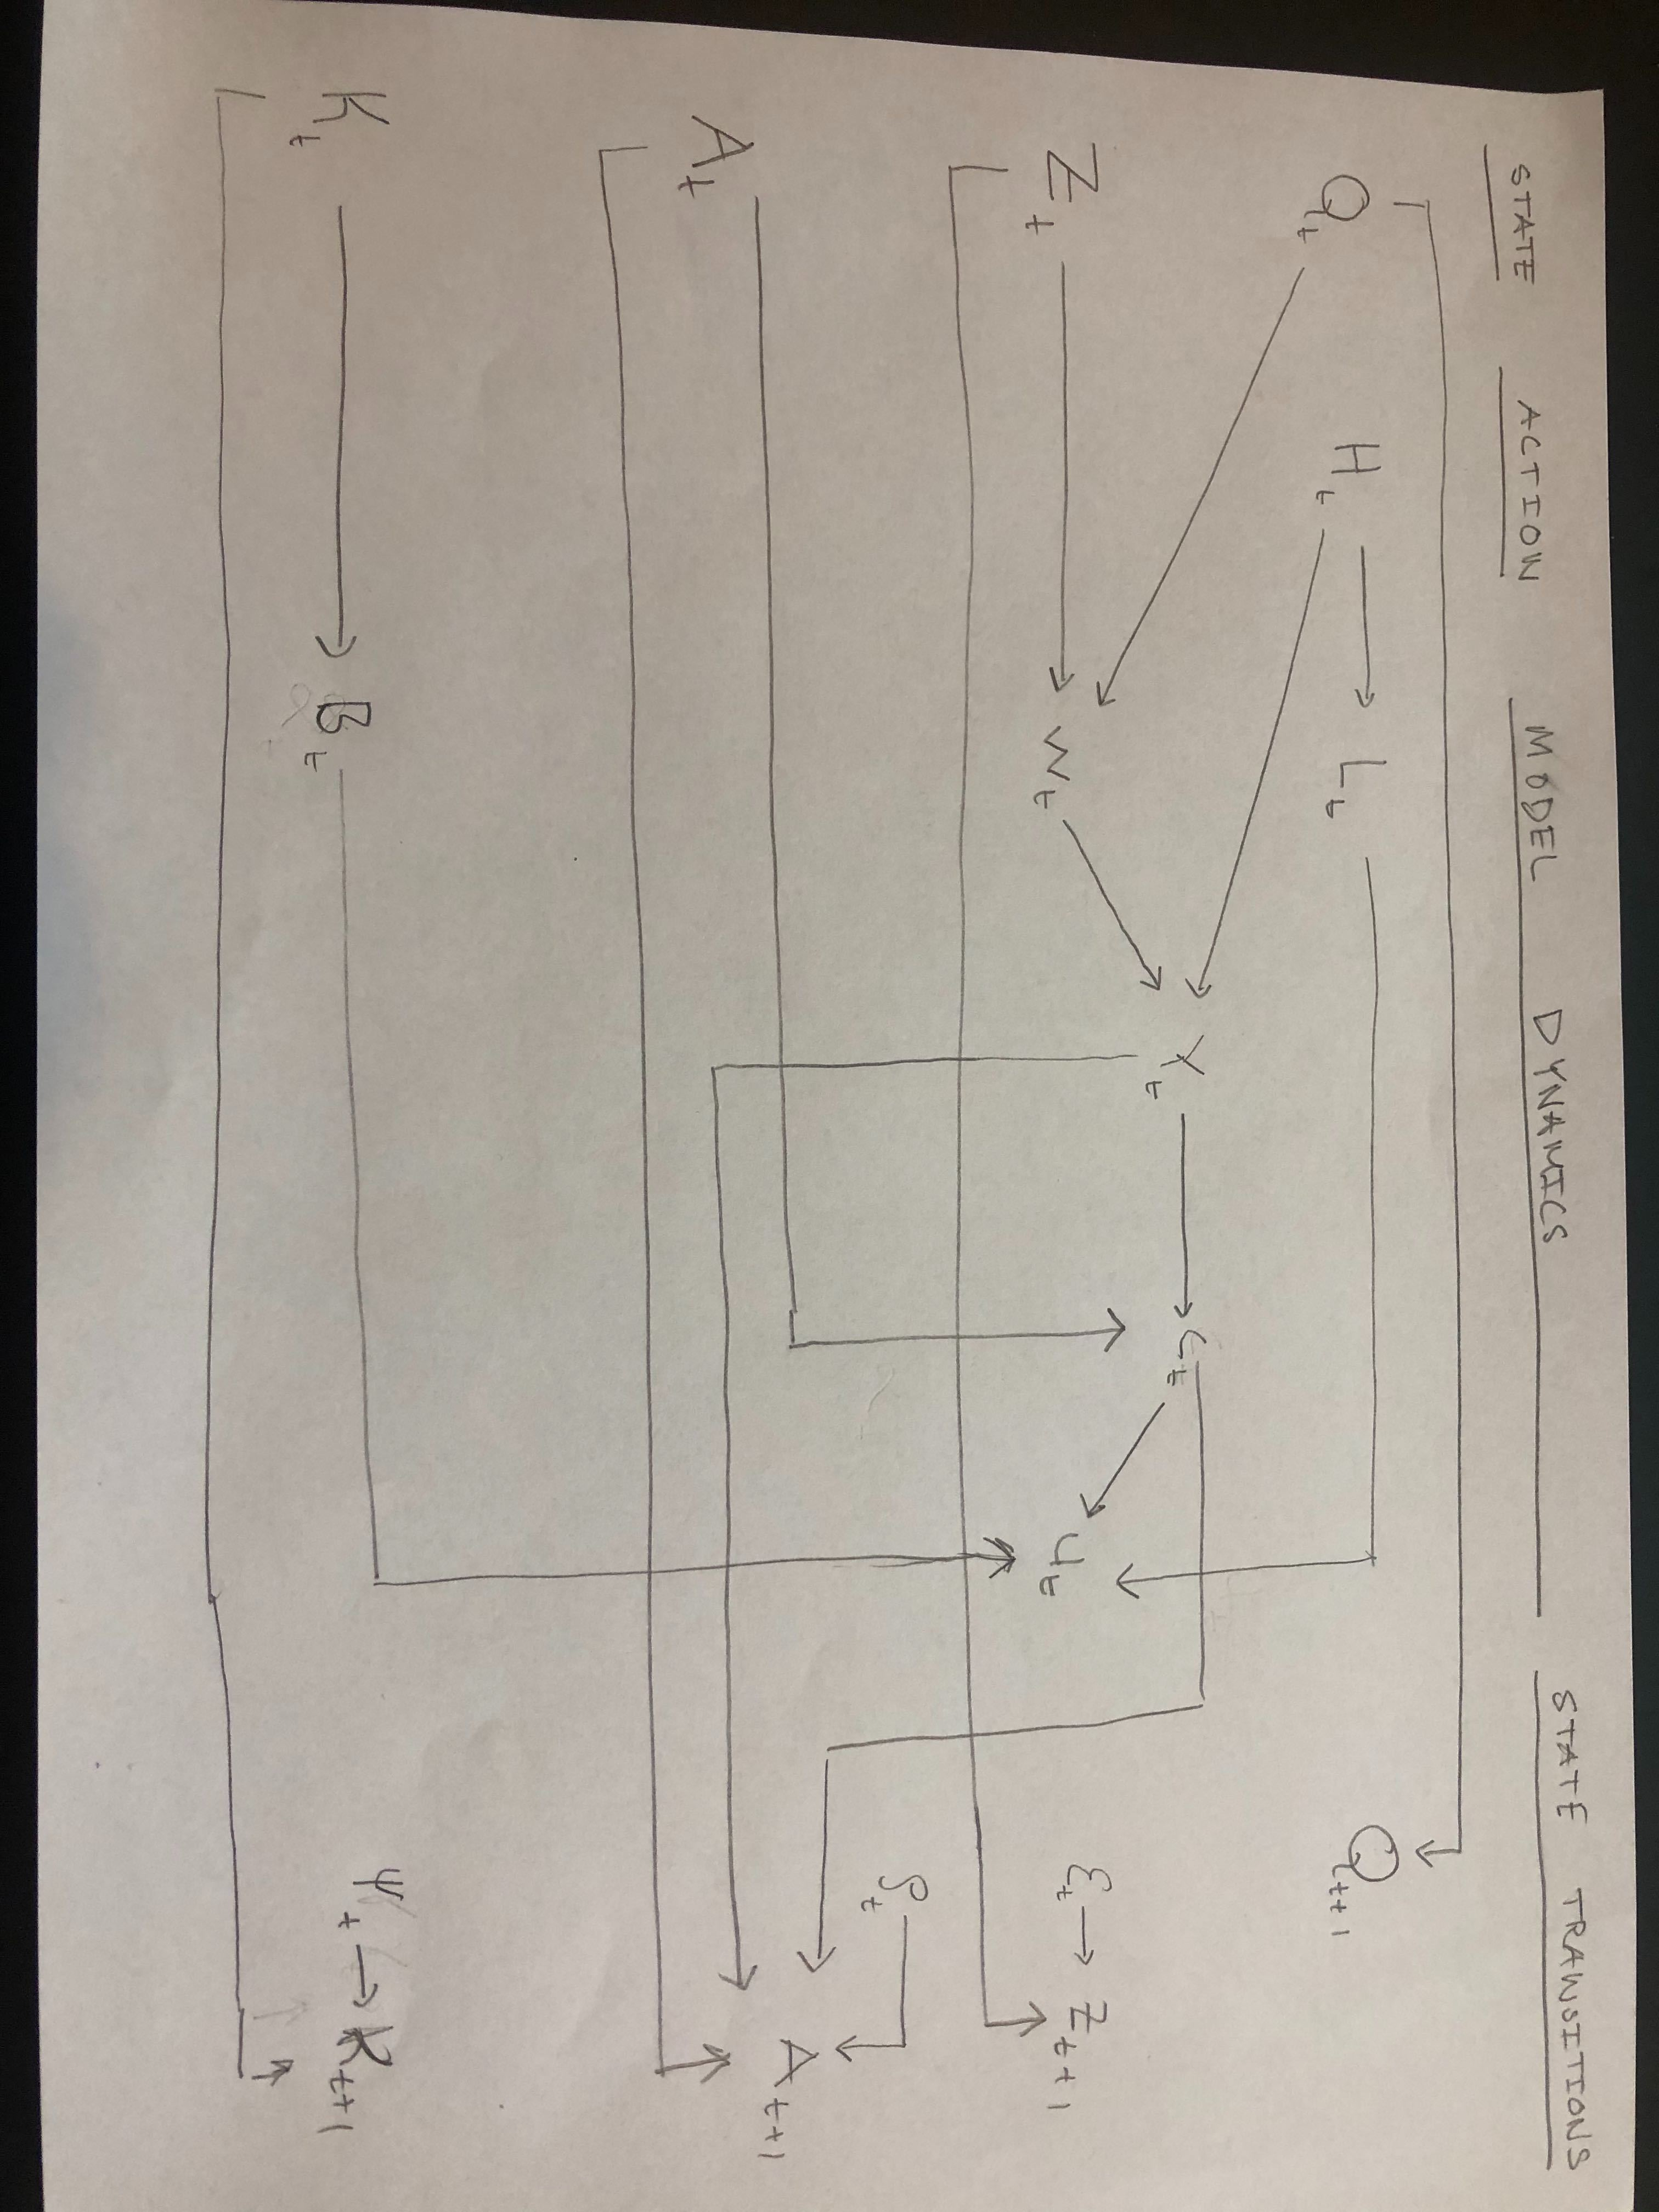
\includegraphics[scale=0.09, angle=90]{figures/modeldynamic_tmp.jpg}
    \caption{Model dynamics (temporary figure) XXX}
    \label{fig:modeldynamics}
\end{figure}

Other variables in the model are: Utility as modelled in equation \eqref{eq:utility_v1} that follow the Cobb-Douglas formulation. Equation \eqref{eq:alpha_v1} denotes the utility dynamic of having kids. Later the functional form of $f^{B}$ is discussed. Equation \eqref{eq:salary_v1} models salary as being the product of the number of working hours and the wage level. \eqref{eq:consumption_v1} is assumed to be fraction of the sum of salary and assets (sometimes referred \textit{cash-on-hand}). \eqref{eq:leisure_v1} shows leisure being the total number of hours in a week - minus the number of hours worked. Equation \eqref{eq:wage_v1} governs how the wage level at time $t$ can be decomposed into an idiosyncratic component and a deterministic component that are deterministic as a function of age.

4 equations govern the law of motion: Equation \eqref{eq:assets_v1} governs how the assets in period $t$ grows with a normally distribution return, adding the salary and subtracting the consumption of period $t$. Equation \eqref{eq:kids_v1} denotes the growth of children. The idiosyncratic wage level is governed by equation \eqref{eq:wage_level_v1}. Where it's assumed that the previous period has influence on the wage level. Equation \eqref{eq:age_v1} shows how the age of the agent follows a deterministic process.

Finally two functions in the formulation should be clearly explicited: $f^{B}, f^{W}$. Starting with $f^{B}$ a couple of things should be noted, about how the function should behave. First and foremost:

\begin{equation}
    f^{B}: \N_{0,+} \mapsto [0,1]
\end{equation}

This is due to the fact that the utility function is of the Cobb-Douglas formulation, where the $B$ parameter should be contained in the interval [0,1]. Second it should be noted that it should not be perfectly determined whether or not:

\begin{equation}
    \frac{d}{d K}f^{B} > 0 \qquad \textbf{or} \qquad \frac{d}{d K}f^{B} < 0
\end{equation}

Therefore the formulation:

\begin{equation}
    f^{B} (K_t)= a + b \frac{\exp{c + d K_t}}{1 + \exp{c + d K_t}}\qquad  \text{s.t. } a + b < 1, a \land b > 0
\end{equation}

The function $f^{W}$ is not parametric, and determined by data from Dansk Statistik XXX.


Parameters of the model being: $\kappa, \mu_\rho, \sigma_\rho, p_\psi, \sigma_\epsilon, \zeta$. and $a, b, c, d$, where the latter govern the dynamic of the utility of leisure conditioned on the number of kids. $\kappa$ governs the consumption profile, $\mu_\rho$ denotes the expected return of the assets, $\sigma_\rho$ the variance. $p_\psi$ is the probability of a new child. $\sigma_{\epsilon}$ is the variance (before the log transformation) of the log-normal shock to the income process. $\zeta$ is growth constant on the wage level evolution.


\textbf{MULIGE UDVIDELSER}: 1) function for $p_\psi (Q_t, K_t)$.  Forbrugs kvotienten $\kappa (Q_t, K_t)$ kan være en funktion af alderen og børn. Man kan også overveje at tilføje transfers. Uddannelses niveayu og dets indflydelse på wage er også en mulighed.
